\documentclass{sig-alternate}
%\usepackage{epstopdf}

\begin{document}

%TODO: cambiar este título horrible
\title{L'Ecuyer y velocidad WARP}

\numberofauthors{2}

\author{
    \alignauthor
    Gomez Vidal, Maximiliano\\
    \email{dgomezvi@alu.itba.edu.ar} \\
    \ \\
    Abramowicz, Pablo\\
    \email{pabramow@alu.itba.edu.ar} \\
    \ \\
    \alignauthor
    Sessa, Carlos\\
    \email{csessa@alu.itba.edu.ar} \\
    \ \\
    Villa Fern\'{a}ndez, Santiago\\
    \email{svillafe@alu.itba.edu.ar}
}

\maketitle

\begin{abstract}
En este art\'{i}culo se analiza el generador de n\'{u}meros pseudo-aleatorios
sugerido por L'Ecuyer y se lo pone a prueba utilizando el test de 
Kolmogorov-Smirnov y el test $\chi^{2}$. Se realiza tambi\'{e}n una simulaci\'{o}n
del tiempo de vuelo de una nave espacial mediante el m\'{e}todo de Montecarlo.
\end{abstract}

\keywords{L'Ecuyer, generador lineal congruencial, simulaci\'{o}n de Montecarlo,
 test $\chi^{2}$, test Kolmogorov-Smirnov, propulsi\'{o}n WARP}

\section{Introducci\'{o}n}\label{introduccion}

El concepto de aleatoriedad est\'{a} presente en diversos campos de la ciencia,
tales como la criptograf\'{i}a y la estad\'{i}stica.

En determinadas ocasiones es deseable generar secuencias de n\'{u}meros
aleatorios. Resulta l\'{o}gico pensar en generar dichas secuencias utilizando
una computadora. Sin embargo, los n\'{u}meros al azar surgen \'{u}nicamente
de procesos naturales que no pueden ser recreados en un dispositivo determinista
como lo es una computadora. La soluci\'{o}n a este problema consiste en utilizar
algoritmos que permitan generar secuencias suficientemente largas de n\'{u}meros
que presenten una distribuci\'{o}n estad\'{i}stica regular. Es decir, que no debe
ser posible distinguir mediante pruebas estad\'{i}sticas que la secuencia no
ha sido construida realmente al azar.

Uno de los generadores m\'{a}s conocidos de n\'{u}meros pseudo-aleatorios es
el generador lineal congruencial (LCG). 

En la secci\'{o}n \ref{generador} se 
analiza el generador de L'Ecuyer, que utiliza dos LCG para generar las secuencias.
En la secci\'{o}n \ref{pruebagenerador} se somete al generador de L'Ecuyer
a tests estad\'{i}sticos para analizar la distribuci\'{o}n de los n\'{u}meros
generados. En la secci\'{o}n \ref{triangular} se obtiene una distribuci\'{o}n
triangular a partir de la salida del generador. En la secci\'{o}n
\ref{simulacionpropulsor} se realiza una simulaci\'{o}n del tiempo de vuelo
de la nave USS Enterprise utilizando el m\'{e}todo de Montecarlo. Finalmente,
se exponen las conclusiones en la secci\'{o}n \ref{conclusiones}.

\section{Generador de L'Ecuyer}\label{generador}

El generador sugerido por L'Ecuyer combina dos LCG de acuerdo al siguiente 
algoritmo:

\textit{PASO 1}
Seleccionar una semilla $X_{1,0}$ en el rango $[1, 2147483562]$ para el LCG$1$
y $X_{2,0}$ en el rango $[1, 2147483398]$ para el LCG$2$.

\textit{PASO 2}
Evaluar cada generador individual

\begin{equation}
\label{LCG1}
X_{1,n+1} = 40014 \ X_{1,n} \ mod \ 2147483563
\end{equation}

\begin{equation}
\label{LCG2}
X_{2,n+1} = 40692 \ X_{2,n} \ mod \ 2147483399
\end{equation}

\textit{PASO 3}
Computar

\begin{equation}
\label{xn}
X_{n+1} = (X_{1,n+1} - X_{2,n+1}) \ mod \ 2147483562
\end{equation}

\textit{PASO 4}
Computar

\begin{equation}
\label{un}
U_{n+1} = 
    \begin{cases}
    \frac{X_{n+1}}{2147483563}, X_{n+1} > 0\\
     \ \\
    \frac{2147483562}{2147483563}, X_{n+1} = 0\\
    \end{cases}
\end{equation}

\textit{PASO 5}
Hacer $n = n + 1$ e ir al \textit{PASO 2}.

\section{Probando el generador de L'Ecuyer}\label{pruebagenerador}

Resulta de inter\'{e}s estudiar si la secuencia generada se encuentra
distribuida de manera uniforme. A continuaci\'{o}n se somete a prueba el
generador de L'Ecuyer utilizando el test $\chi^{2}$ y el test de 
Kolmogorov-Smirnov.

\subsection{Test $\chi^{2}$}\label{testchicuadrado}

Se desea establecer si es posible aceptar la hip\'{o}tesis $H_{0}:$ la secuencia
generada utilizando el algoritmo de la secci\'{o}n \ref{generador} corresponde 
a muestras de una variable uniforme $\mathcal{U}[0,1)$,
con un nivel de confianza del $95\%$. Para esto se generan $10,000$ n\'{u}meros 
utilizando $(0,2)$ como semillas. Luego se agrupan en $100$ intervalos de clase.

La media esperada en cada intervalo de clase es $E_{i} = 100$, pues se analiza 
una distribuci\'{o}n uniforme. El estad\'{i}stico dado por la ecuaci\'{o}n:

\begin{equation}\label{estadistico}
\chi^{2}_{0} = \sum_{i=1}^{100} \frac{(O_{i} - E_{i})^{2}}{E_{i}}
\end{equation}

resulta aproximadamente $98.84$.
Se observa que la distribuci\'{o}n $\chi^{2}$ subyacente posee $99$ grados de
libertad, puesto que se han considerado $100$ categor\'{i}as para agrupar los
n\'{u}meros generados.

Para el nivel de significaci\'{o}n deseado, $\alpha = 0.05$, se obtiene el
valor cr\'{i}tico $\chi^{2}_{99,0.05} = 124.3421$. Como 
$\chi^{2}_{99,0.05} > \chi^{2}_{0}$ se acepta $H_{0}$ y se determina que
los n\'{u}meros est\'{a}n distribuidos de manera uniforme. En la figura
~\ref{fig:clases} se observa la distribuci\'{o}n de los $10,000$ n\'{u}meros para
cada clase. En las figuras ~\ref{fig:duplas} y ~\ref{fig:ternas} se observa que no es
posible detectar patrones en la distribuci\'{o}n de la secuencia generada, puesto
que la misma presenta una densidad uniforme.

%Aca estaban los graficos antes

\subsection{Test Kolmogorov-Smirnov}\label{testks}

Este test se utiliza para contrastar uniformidad. Compara la distribuci\'{o}n
emp\'{i}rica obtenida a partir de una muestra con la distribuci\'{o}n te\'{o}rica
correspondiente a la variable aleatoria en estudio.

Se mantienen los mismos $10,000$ n\'{u}meros generados en la secci\'{o}n
\ref{testchicuadrado} y la misma hip\'{o}tesis $H_{0}$. Se agrupan los n\'{u}meros
nuevamente en $100$ intervalos. Se realiza el test
correspondiente comparando la secuencia arrojada por el generador de L'Ecuyer
con otra muestra que presenta una distribuci\'{o}n uniforme. 

El resultado
arrojado es una aceptaci\'{o}n de $H_{0}$ con aproximadamente un $96.45\%$
de confianza, por lo que no se rechaza la hip\'{o}tesis nula a un nivel de 
significaci\'{o}n de 0.05. Es decir, la secuencia generada presenta una 
distribuci\'{o}n uniforme.

\section{Densidad triangular}\label{triangular}

En los experimentos de simulaci\'{o}n es necesario generar secuencias de
n\'{u}meros pseudo-aleatorios distribuidos de acuerdo a una funci\'{o}n $F(x)$
arbitraria.

A continuaci\'{o}n se utiliza la t\'{e}cnica de la transformada inversa
aplicada a la funci\'{o}n de densidad triangular dada por:

\begin{equation}
\label{triangularEc}
f_{X}(x) = 
    \begin{cases}
    \frac{2(x-a)}{(b-a)(c-a)}, &  a \le x \le b\\
     \ \\
    \frac{2(c-x)}{(c-b)(c-a)}, & b < x \le c\\
     \ \\
     0, & \text{en otro lado}\\
    \end{cases}
\end{equation}

Esta t\'{e}cnica establece que dado un n\'{u}mero $u$ que es una realizaci\'{o}n
de $\mathcal{U} \sim \mathcal{U}[0,1]$, entonces $F^{-1}(u)$ es una
realizaci\'{o}n de una variable aleatoria $X$ con funci\'{o}n de distribuci\'{o}n
$F(x)$.

Integrando la ecuaci\'{o}n \ref{triangularEc} se obtiene la funci\'{o}n de 
distribuci\'{o}n $F_{X}(x)$:

\begin{equation}
\label{triangularIntegrada}
F_{X}(x) = 
    \begin{cases}
    0, & x < a\\
     \ \\
    \frac{x^{2} - 2ax + a^{2}}{(b-a)(c-a)}, &  a \le x \le b\\
     \ \\
    \frac{b-a}{c-a} + \frac{2cx - x^{2} - b(2c-b)}{(c-b)(c-a)}, & b < x \le c\\
     \ \\
     1, & x > c\\
    \end{cases}
\end{equation}

Por \'{u}ltimo, la VA $X$ resulta:

\begin{equation}
\label{vaconftriangular}
X = 
    \begin{cases}
    a + \sqrt{U(c-a)(b-a)}, 0 \leq U \leq \frac{b-a}{c-a} \\
    \ \\
    c + \sqrt{(c-b)^{2} - U(c-b)(c-a) + (b-a)(c-b)}, \\ \frac{b-a}{c-a} < U \leq 1 \\
    \end{cases}
\end{equation}

%En la figura ~\ref{fig:triangular} se observa la distribuci\'{o}n para los
%valores $a = 0$, $b = 1$ y $c = 3$.

\section{Sistema de propulsi\'{o}n WARP}\label{simulacionpropulsor}
El sistema de propulsi\'on WARP de la nave espacial USS Enterprise consiste en un n\'ucleo WARP
en el interior de un reactor donde se llevan a cabo reacciones de aniquilaci\'on 
materia-antimateria, moderadas por cristales de Dilitio. Dichos cristales se
procesan en una c\'amara controlada llamada Matriz de Dilitio, el cual tiene
un subsistema de redundancia. Este proceso se realiza para alimentar a los 
propulsores en las nescellas laterales de la nave. El tiempo de operaci\'on de 
cada propulsor es una variable aleatoria exponcialmente distribuida $X_1$,  $X_2$ 
con tiempo medio $T_m = 240$ horas. El tiempo de operaci\'on entre fallos del n\'ucleo 
WARP es una variable uniforme $X_3 \sim \mathcal{U}[72,12]$, el tiempo de operaci\'on 
de la c\'amara de Dilitio es una variable uniforme $X_4 \sim \mathcal{U}[20,30]$ y, por 
\'ultimo, el tiempo entre fallos de la c\'amara de redundacia es una variable uniforme 
$X_5 \sim \mathcal{U}[5,7]$, todas medidas en horas.

Las funciones de distribuci\'on se describen como:

Siendo $x_1$ y $x_2$ realizaciones de $X_1$ y $X_2$:
\begin{equation}
	f_{x_1, x_2}(t) = 
		\begin{cases}
		  \frac{1}{T_m} e^{-\frac{t}{T_m}} & t > 0 \\
		  0 & t < 0
		\end{cases}
\end{equation}

Siendo $x_3$ una realizaci\'on de $X_3$:
\begin{equation}
	f_{x_3}(x) = 
		\begin{cases}
		  \frac{1}{12} & x \in (72,84) \\
		  0 & x \notin (72,84)
		\end{cases}
\end{equation}

Siendo $x_4$ una realizaci\'on de $X_4$:
\begin{equation}
	f_{x_4}(x) = 
		\begin{cases}
		  \frac{1}{30} & x \in (20,50) \\
		  0 & x \notin (20,50)
		\end{cases}
\end{equation}

Siendo $x_5$ una realizaci\'on de $X_5$:
\begin{equation}
	f_{x_5}(x) = 
		\begin{cases}
		  \frac{1}{7} & x \in (5,12) \\
		  0 & x \notin (5,12)
		\end{cases}
\end{equation}

El tiempo de operaci\'on del sistema integrado es una variable 
aleatoria $T$ definida como:

\begin{equation}
 T = \min\{ \max \{ X_4, X_5 \} , X_3 , \max \{X_2, X_1\}\}
\end{equation}

Cuyo tiempo medio entre fallos del sistema se describe de la forma:
\begin{eqnarray}
\label{integralsintrans}
	\mathcal{E} \{ T \} = \int\limits_{\mathcal{D}} \min\{ \max \{ x_4, x_5 \} , x_3 , \max \{x_2, x_1\}\}
	\nonumber
	\\
	f_{x_1}(x_1) f_{x_2}(x_2) f_{x_3}(x_3) f_{x_4}(x_4) f_{x_5}(x_5) d^5x
\end{eqnarray}
donde $\mathcal{D}$ es el dominio $[5,12]$ x $[20,50]$ x $[72,84]$ x $[0,\infty]$ x $[0,\infty]$.

Se transforma el dominio de integraci\'on $\mathcal{D} \to [0,1]^5$ de manera de poder 
realizar la simulaci\'on de Montecarlo para este sistema. Las transformaciones se definen como:

\begin{eqnarray}
	\label{trans_uno}
	x_1 = - T_m \ln (1 - u_1) \\
	\label{trans_dos}
	x_2 = - T_m \ln (1 - u_2) \\
	\label{trans_tres}
	x_3 = 12 u_3 + 72 \\
	\label{trans_cuatro}
	x_4 = 30 u_4 + 20 \\
	\label{trans_cinco}
	x_5 = 5 u_5 + 7
\end{eqnarray}
siendo $u_i$ realizaciones de variables aleatorias $\mathcal{U}[0,1]$.

Se obtiene el determinante jacobiano de la transformaci\'on:
\begin{equation}
	\label{jacobiano}
	J =
		\begin{vmatrix}
			\frac{T_m}{1 - u_1} & 0  & 0  & 0  & 0 \\
			0 & \frac{T_m}{1 - u_2} & 0  & 0  & 0  \\
			0 & 0 & 12 & 0 & 0 \\
			0 & 0 & 0 & 30  & 0 \\
			0 & 0 & 0 & 0 & 5 \\
		\end{vmatrix}
	=
		\frac{180 T_m^2}{(1-u_1)(1-u_2)}
\end{equation}

Por \'ultimo se reemplaza en \eqref{integralsintrans} con
\eqref{trans_uno}, \eqref{trans_dos}, \eqref{trans_tres}, \eqref{trans_cuatro}, \eqref{trans_cinco}, 
se multiplica por \eqref{jacobiano}, y se obtiene la integral transformada:

\begin{eqnarray}
\label{integralcontrans}
	\mathcal{E} \{ T \} =	\int\limits_{[0,1]^6} \min\{ \max \{ 30 u_4 + 20, 5 u_5 + 7 \} , 12 u_3
	\nonumber
	\\
	 + 72 , \max \{- T_m \ln (1 - u_2), - T_m \ln (1 - u_1)\}\} d^5u
\end{eqnarray}

Para la realizaci\'on de la simulaci\'on del sistema mediante el m\'etodo de Montecarlo 
se utiliza el generador de n\'umeros pseudo-aleatorios de L'Ecuyer obtenido en la secci\'on \ref{pruebagenerador},
calculando 5 secuencias correspondientes a $u_i \in [0,1]$. Se realizan 20 simulaciones  
de la integral \eqref{integralcontrans}, resultando el
estimador de tiempo medio de vuelo $\langle T \rangle = 34.798822$ horas y el desv\'io muestral
$S = 0.86899$ horas. Se determina que para un nivel de significaci\'on del $5\%$, el tiempo medio de vuelo
del sistema de propulsi\'on WARP pertenece al rango $ 34.80 \pm 0.406 $ horas.

\begin{table}[h]
\label{seeds}
\centering
\begin{tabular}{|c|c|c|}
\hline
 $u_1$ & 13 & 20 \\
\hline
 $u_2$ & 52 & 87 \\
\hline
 $u_3$ & 101 & 115 \\
\hline
\end{tabular}
\caption{Semillas para los generadores de L'Ecuyer de $u_i$}
\end{table}


\section{Conclusiones}\label{conclusiones}

A partir de las simulaciones y los tests que se realizan al generador de n\'{u}meros 
aleatorios de L'Ecuyer se desprende que es un buen generador, ya que no solo no 
se observan hiperplanos en los gr\'{a}ficos sino que tambi\'{e}n fue sometido a
los tests $\chi^{2}$ y Kolmogorov-Smironov con resultado exitoso. Este generador
permite realizar diversas simulaciones con la seguridad de que los datos de
entrada presentan una distribuci\'{o}n uniforme.
%En lo que respecta al USS Enterprise

\begin{figure*}[hp]
\centering
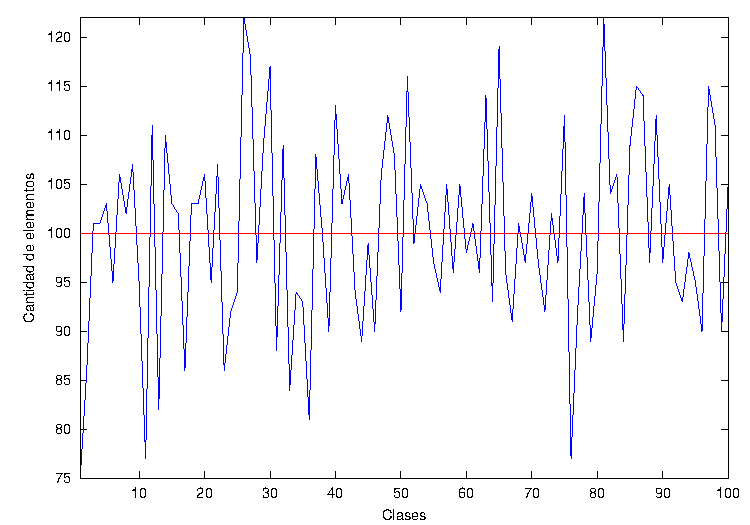
\includegraphics[scale=0.8]{graficos/clases}
\caption{Cantidad de resultados por categor\'{i}a para el test $\chi^{2}$}
\label{fig:clases}
\end{figure*}

\begin{figure*}[hp]
\centering
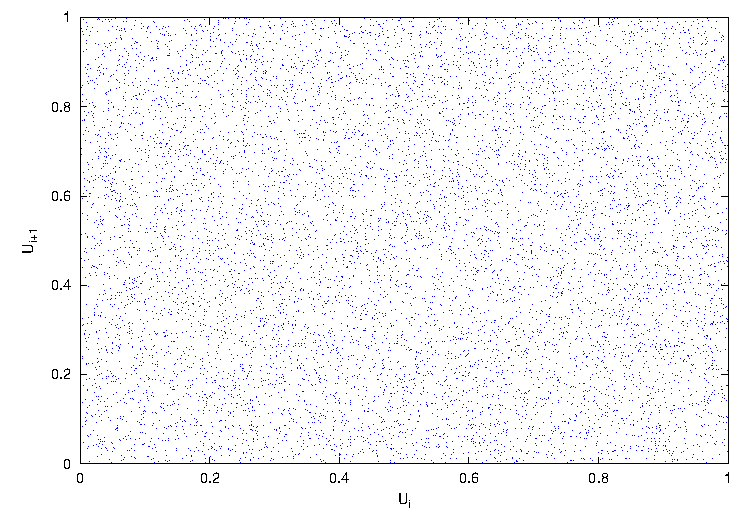
\includegraphics[scale=0.8]{graficos/duplas}
\caption{Duplas $(U_{i}, U_{i+1})$ de n\'{u}meros pseudo-aleatorios generados}
\label{fig:duplas}
\end{figure*}

\begin{figure*}[hp]
\centering
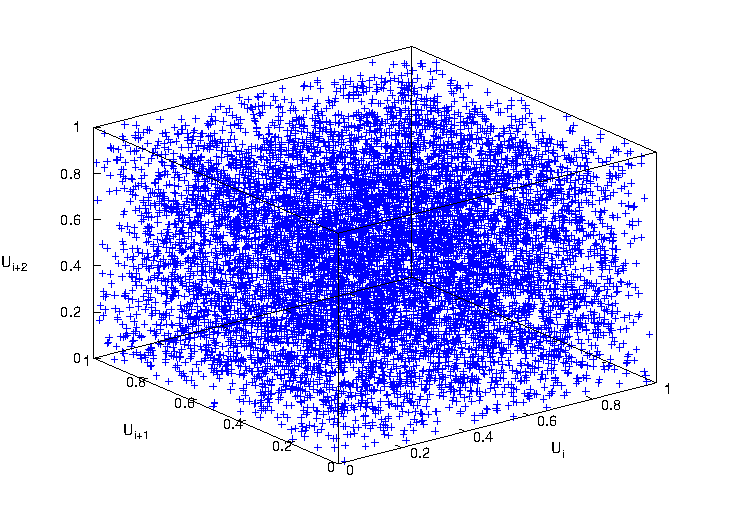
\includegraphics[scale=0.8]{graficos/ternas}
\caption{Ternas $(U_{i}, U_{i+1}, U_{i+2})$ de n\'{u}meros pseudo-aleatorios
generados}
\label{fig:ternas}
\end{figure*}

\end{document}
